\section{Evaluating the unfairness of Atomic Swaps}
\label{sec:evaluation}

In this section, we evaluate the unfairness of Atomic Swaps.
In particular, our evaluation consists of two parts: quantifying the unfairness and estimating the unpaid premium.
Quantifying the unfairness is based on analyzing the historical exchange rate volatility, while estimating the unpaid premium is based on the Cox-Ross-Rubinstein option pricing model - the conventional option pricing model for American-style options.
Furthermore, we also evaluate conventional financial assets - the stocks and the currency exchanges - and compare their results with cryptocurrencies.

\subsection{Experimental setting}

We collected relevant data of mainstream cryptocurrencies for one year, starting from May 3th 2018 to May 3th 2019.
In particular, the cryptocurrency exchange rate data was retrieved from from CoinGecko~\footnote{\url{https://www.coingecko.com}.};
the stock index data was retrieved from Yahoo Finance~\footnote{\url{https://finance.yahoo.com}.};
the currency exchange rate data was retrieved from Investing.com~\footnote{\url{https://www.investing.com}.}.

All experiments run on a MacBook Pro with a 2.2 GHz Intel Core i7 Processor, a 16 GB DDR4 RAM and 256 SSD storage disk.

\subsection{Quantifying the unfairness by market volatility}
\label{subsec:volatility_analysis}

We start from identifying the unfairness of Atomic Swaps before evaluating it.
The unfairness consists of two parts as shown in Figure~\ref{fig:unfair_diagram}, namely the profit when the initiator's asset price rises and the mitigated loss when the initiator's asset price drops.

\begin{figure}
    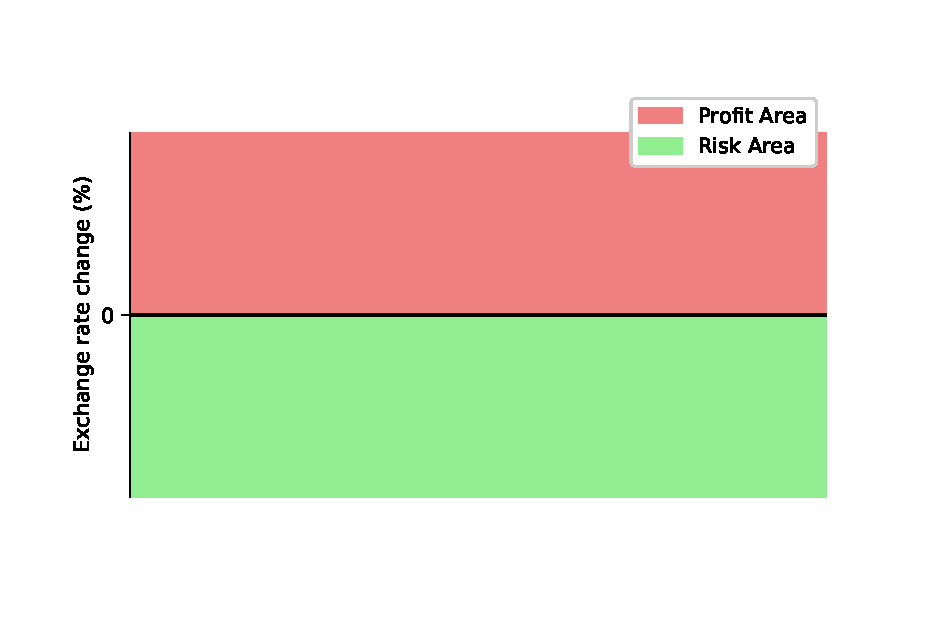
\includegraphics[width=\linewidth]{unfair_diagram.eps}
    \caption{Visualizing the unfairness. The x-axis is time (in days), and the y-axis is the exchange rate change in percentage. For a point $(x, y)$, if $y > 0$, the point falls to the profit area (the red area on the figure), and the Atomic Swap initiator will profit $y$ today. If $y < 0$ the point falls to the risk area (the red area on the figure), and the Atomic Swap initiator will mitigate the loss of $y$ today.}
    \label{fig:unfair_diagram}
\end{figure}

We then quantifying it by using the historical data.

% scenario
\paragraph{Quantifying the unfairness.}
Recall that 24 hours is the default timelock period of the participant,
and the initiator has advantage over the participant within the timelock of 24 hours.
We assume the initiator launches an atomic swap with the value of $x$ USD every day.
For each day, the initiator may either profit a percent $\alpha$ of $x$ directly if his asset price rises,
or mitigate a percent $\beta$ of $x$ by aborting the swap if his asset price drops on average.
Assume the possibility for the initiator's asset price to rise is $P_{\alpha}$, and to drop is $P_{\beta}$.
Then, the expected profit rate is $E_{\alpha} = \alpha P_{\alpha}$,
and the expected mitigated risk rate is $E_{\beta} = \beta P_{\beta}$.
Therefore, the expected unfairness is that the initiator profits $E_{\alpha} x$ unconditionally and mitigates the risk of losing $E_{\beta} x$.
Also, as $E_\alpha$ and $E_\beta$ are equally calculated, they can be added together to derive the total unfairness as $E_\alpha + E_\beta$.

\paragraph{Experimental methodology.}
In our scenario, quantifying the unfairness is to estimate $E_{\alpha}$ and $E_{\beta}$.
We estimate $E_{\alpha}$ and $E_{\beta}$ for each selected cryptocurrency pair.
Furthermore,  we also evaluate the unfairness of stocks and fiat currencies in the same setting, in order to make comparisons.
We use S\&P500 and Dow Jones Index (DJI) as examples of stocks, and USD-EUR and USD-GBP as examples of fiat currencies.

\paragraph{Results and analysis.}

\begin{figure*}
    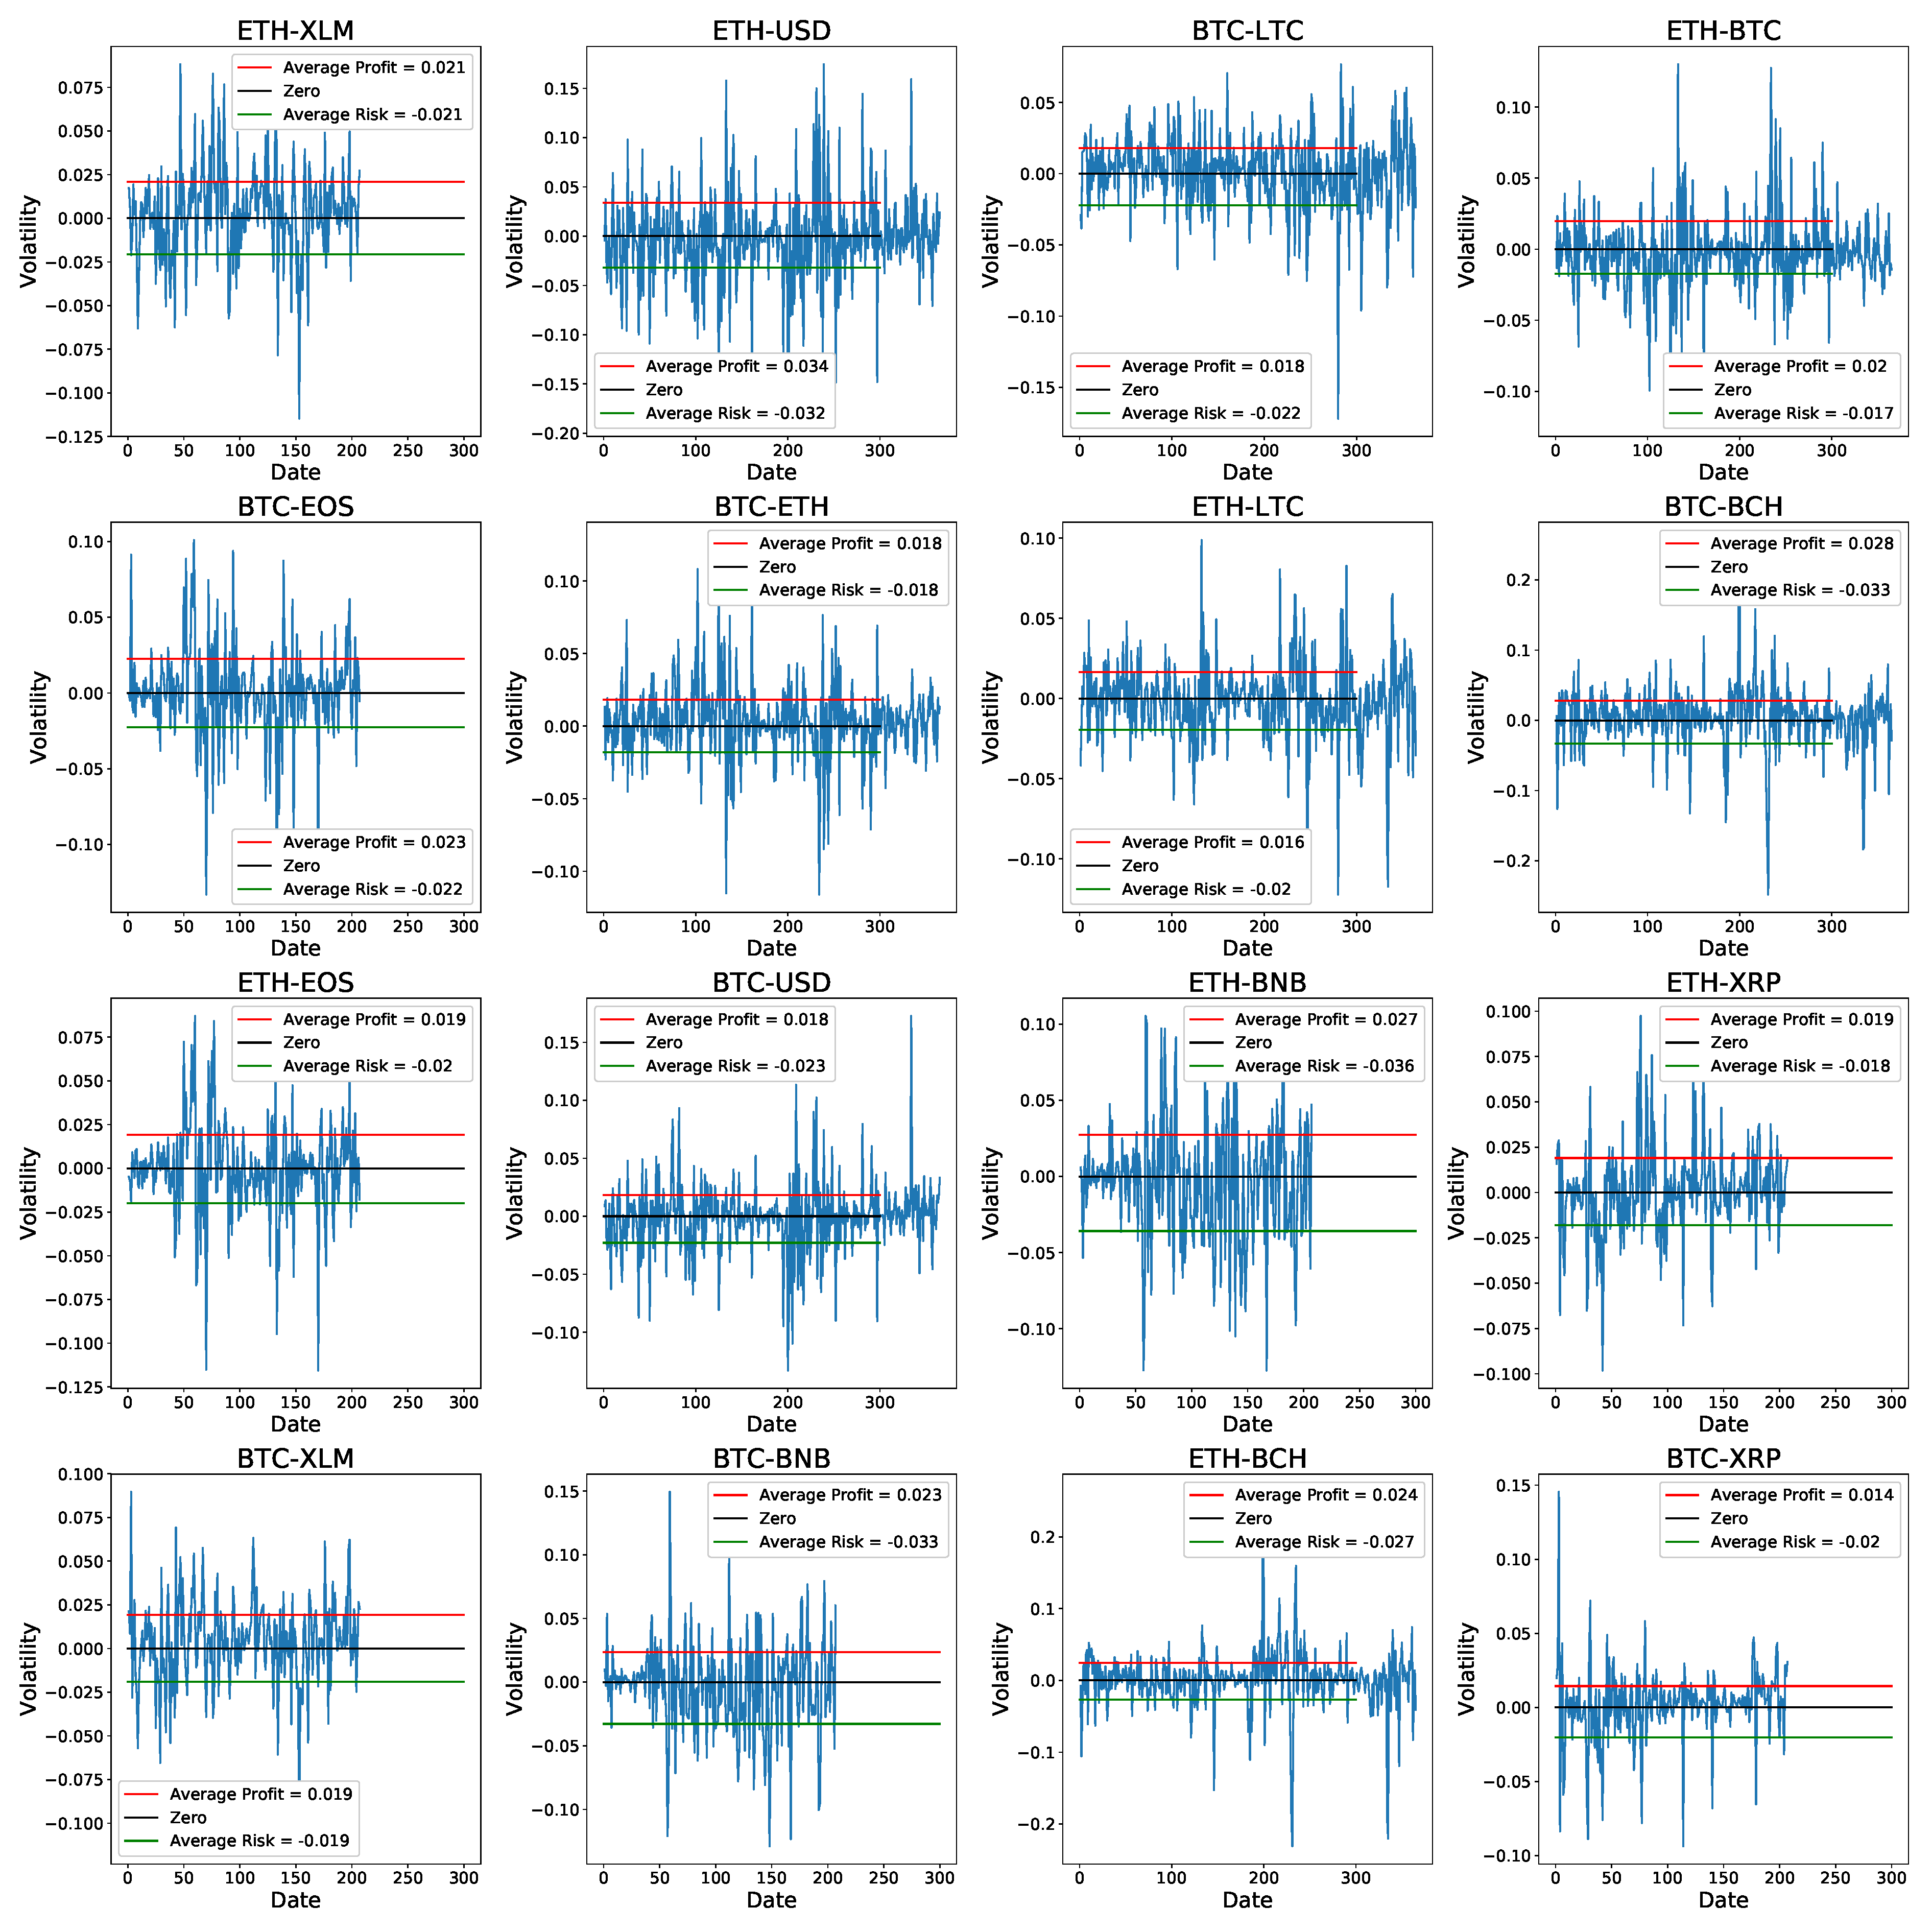
\includegraphics[width=\linewidth]{volatility_analysis.eps}
    \caption{The daily percentage changes for all selected cryptocurrency pairs, stock indices and fiat currency pairs over one year (from 03/05/2018 to 03/05/2019). For each figure, $E_{\alpha}$, $E_{\beta}$, $max_\alpha$ and $max_\beta$ are the expected profit rate, the expected mitigated risk rate, the maximum daily profit and the maximum daily mitigated risk, respectively.}
    \label{fig:volatility_analysis}
\end{figure*}

\begin{figure}
    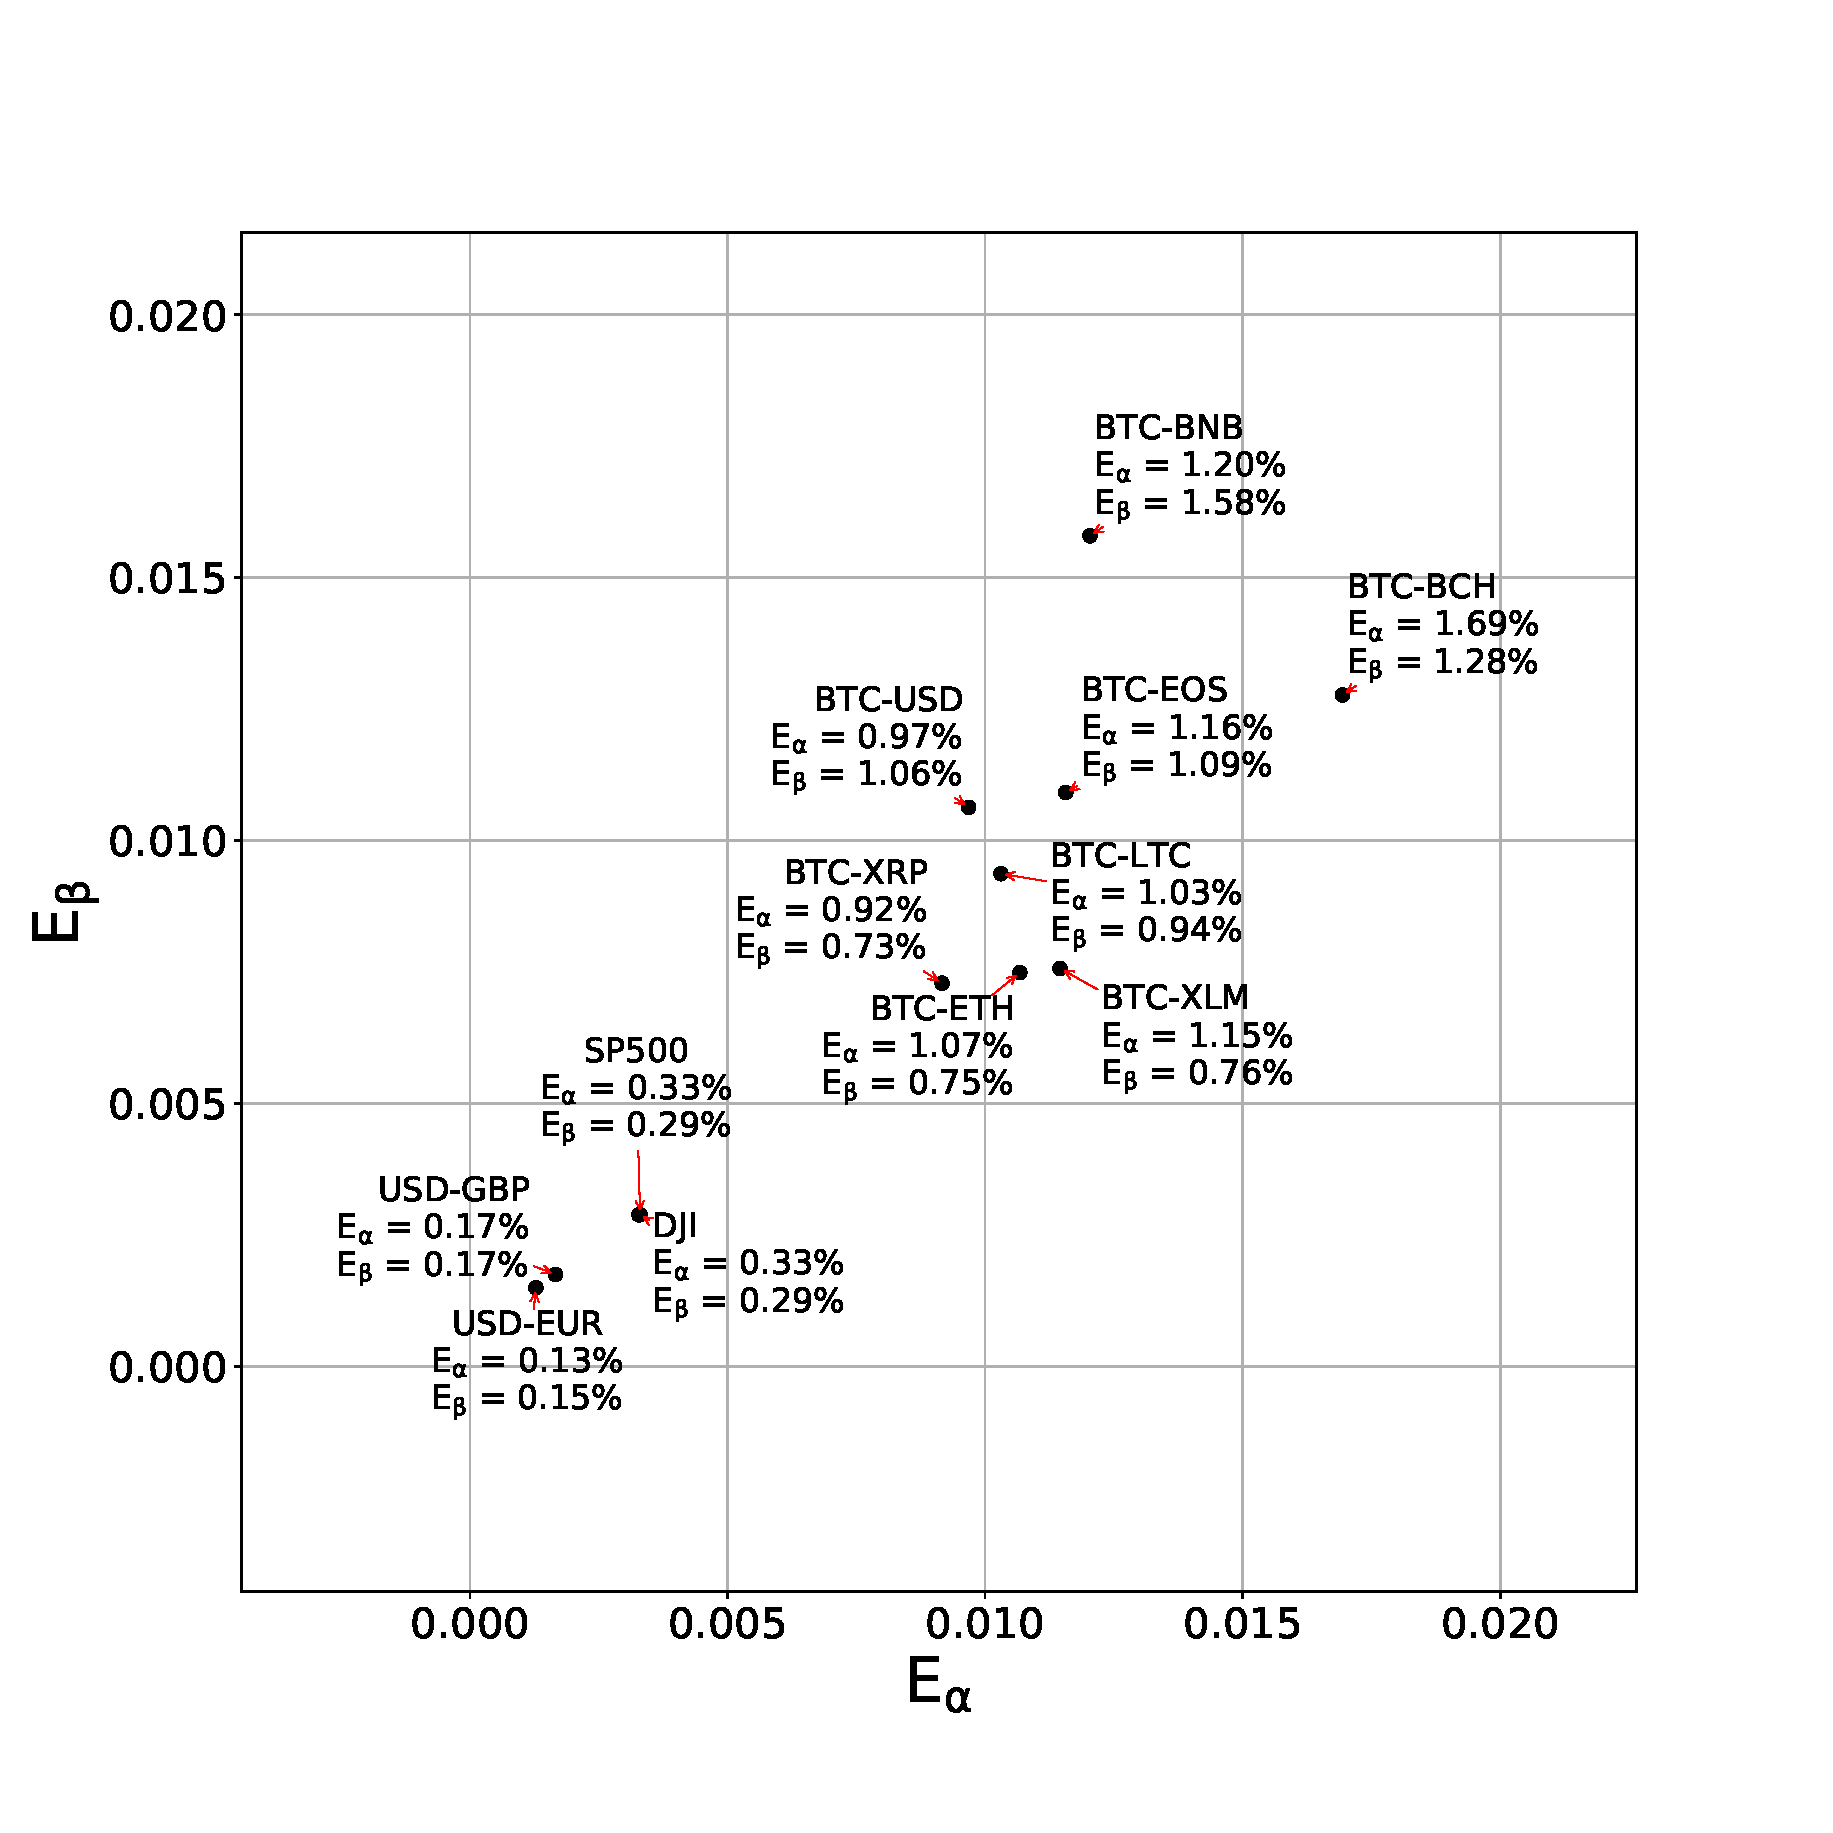
\includegraphics[width=\linewidth]{vol_scatter.eps}
    \caption{Visualizing the expected profit rate $E_\alpha$ and the expected mitigated risk rate $E_\beta$ for each cryptocurrency pair, stock index and fiat currency pair.}
    \label{fig:vol_scatter}
\end{figure}

Figure~\ref{fig:volatility_analysis} shows the estimated $E_\alpha$, $E_\beta$, the maximum daily rises $max_\alpha$ and the maixmum daily drops $max_\beta$ for chosen 8 cryptocurrency pairs, stock indices (S\&P500 and DJI) and fiat currency exchange rates (USD-EUR and USD-GBP).
Figure~\ref{fig:vol_scatter} visualizes $E_\alpha$ and $E_\beta$ of all evaluated items in Figure~\ref{fig:volatility_analysis}.

\TODO{analysis may be improved}
We observe that for all chosen cryptocurrency pairs, $max_\alpha$ and $max_\beta$ are quite big - ranging from 8\% to 25\%.
Meanwhile, $max_\alpha$ and $max_\beta$ of stock indices are much smaller than all cryptocurrency pairs,
and $max_\alpha$ and $max_\beta$ of fiat currencies are even smaller than stock indices.
This indicates that in the setting of an 24-hour Atomic Swap, the cryptocurrency is much more unfair than stocks, and the stocks are more unfair than fiat currencies.

Also, for all chosen cryptocurrency pairs, $E_{\alpha}$ and $E_{\beta}$ are near and the value is approximately 1\%, ranging from 0.73\% to 1.69\%.
For stock indices, the results of S\&P500 and DJI are the same - $E_\alpha = 0.33\%$ and $E_\beta = 0.29\%$, which are smaller than cryptocurrency pairs.
For fiat currencies, $E_\alpha$ and $E_\beta$ are even smaller than stock indices: The value ranges from 0.13\% to 0.17\%.
In addition to the unfairness results like the previous observation, we quantify the unfairness of Atomic Swaps for cryptocurrency pairs: It ranges from  1.65\% (BTC-XRP) to 2.97\% (BTC-BCH).



















\subsection{Estimating the unpaid premium}

To make the Atomic Swap fair, the initiator should pay for the premium.
In other words, the unfair part of the Atomic Swap is the unpaid premium from the initiator.
We evaluate the unfairness of the Atomic Swap by estimating the premium.

As the premium is the only variable in an option contract, estimating the premium is also called the ``Option Pricing'' problem.
In finance, the Black-Scholes (BS) Model is utilized to price the European Call Options,
while the Cox-Ross-Rubinstein (CRR) Model is utilized to price the American Call Options.
Therefore, we utilize the CRR Model to evaluate the unfairness of the Atomic Swap.

\subsubsection{The Cox-Ross-Rubinstein Model Explained}

The CRR Model, which is also called the Binomial Options Pricing Model (BOPM), provides a generalizable numerical method for pricing the options.
Intuitively, the CRR model enumerates all possible prices of the asset in the near future based on the price volatility,
then reverse-engineers the option price based on the enumerated prices.
% binomial tree
Enumerating the possible prices utilizes a binomial tree, where each node represents a point of time.
The model assume that for each step on the binomial tree, the price rises or falls by a fixed rate.
% reverse engineering
Reverse engineering the option price relies on iteratively back propagating the option price for each level of the binomial tree.

Formally, pricing the American Call Option $\Pi = (\pi_1, \pi_2, K, A, T, C)$ by using the CRR model is as follows:

\begin{enumerate}
    \item Creating the binomial price tree
    \item Finding the option prices for leaf nodes
    \item Finding the option prices for earlier nodes 
\end{enumerate}


\begin{figure}
    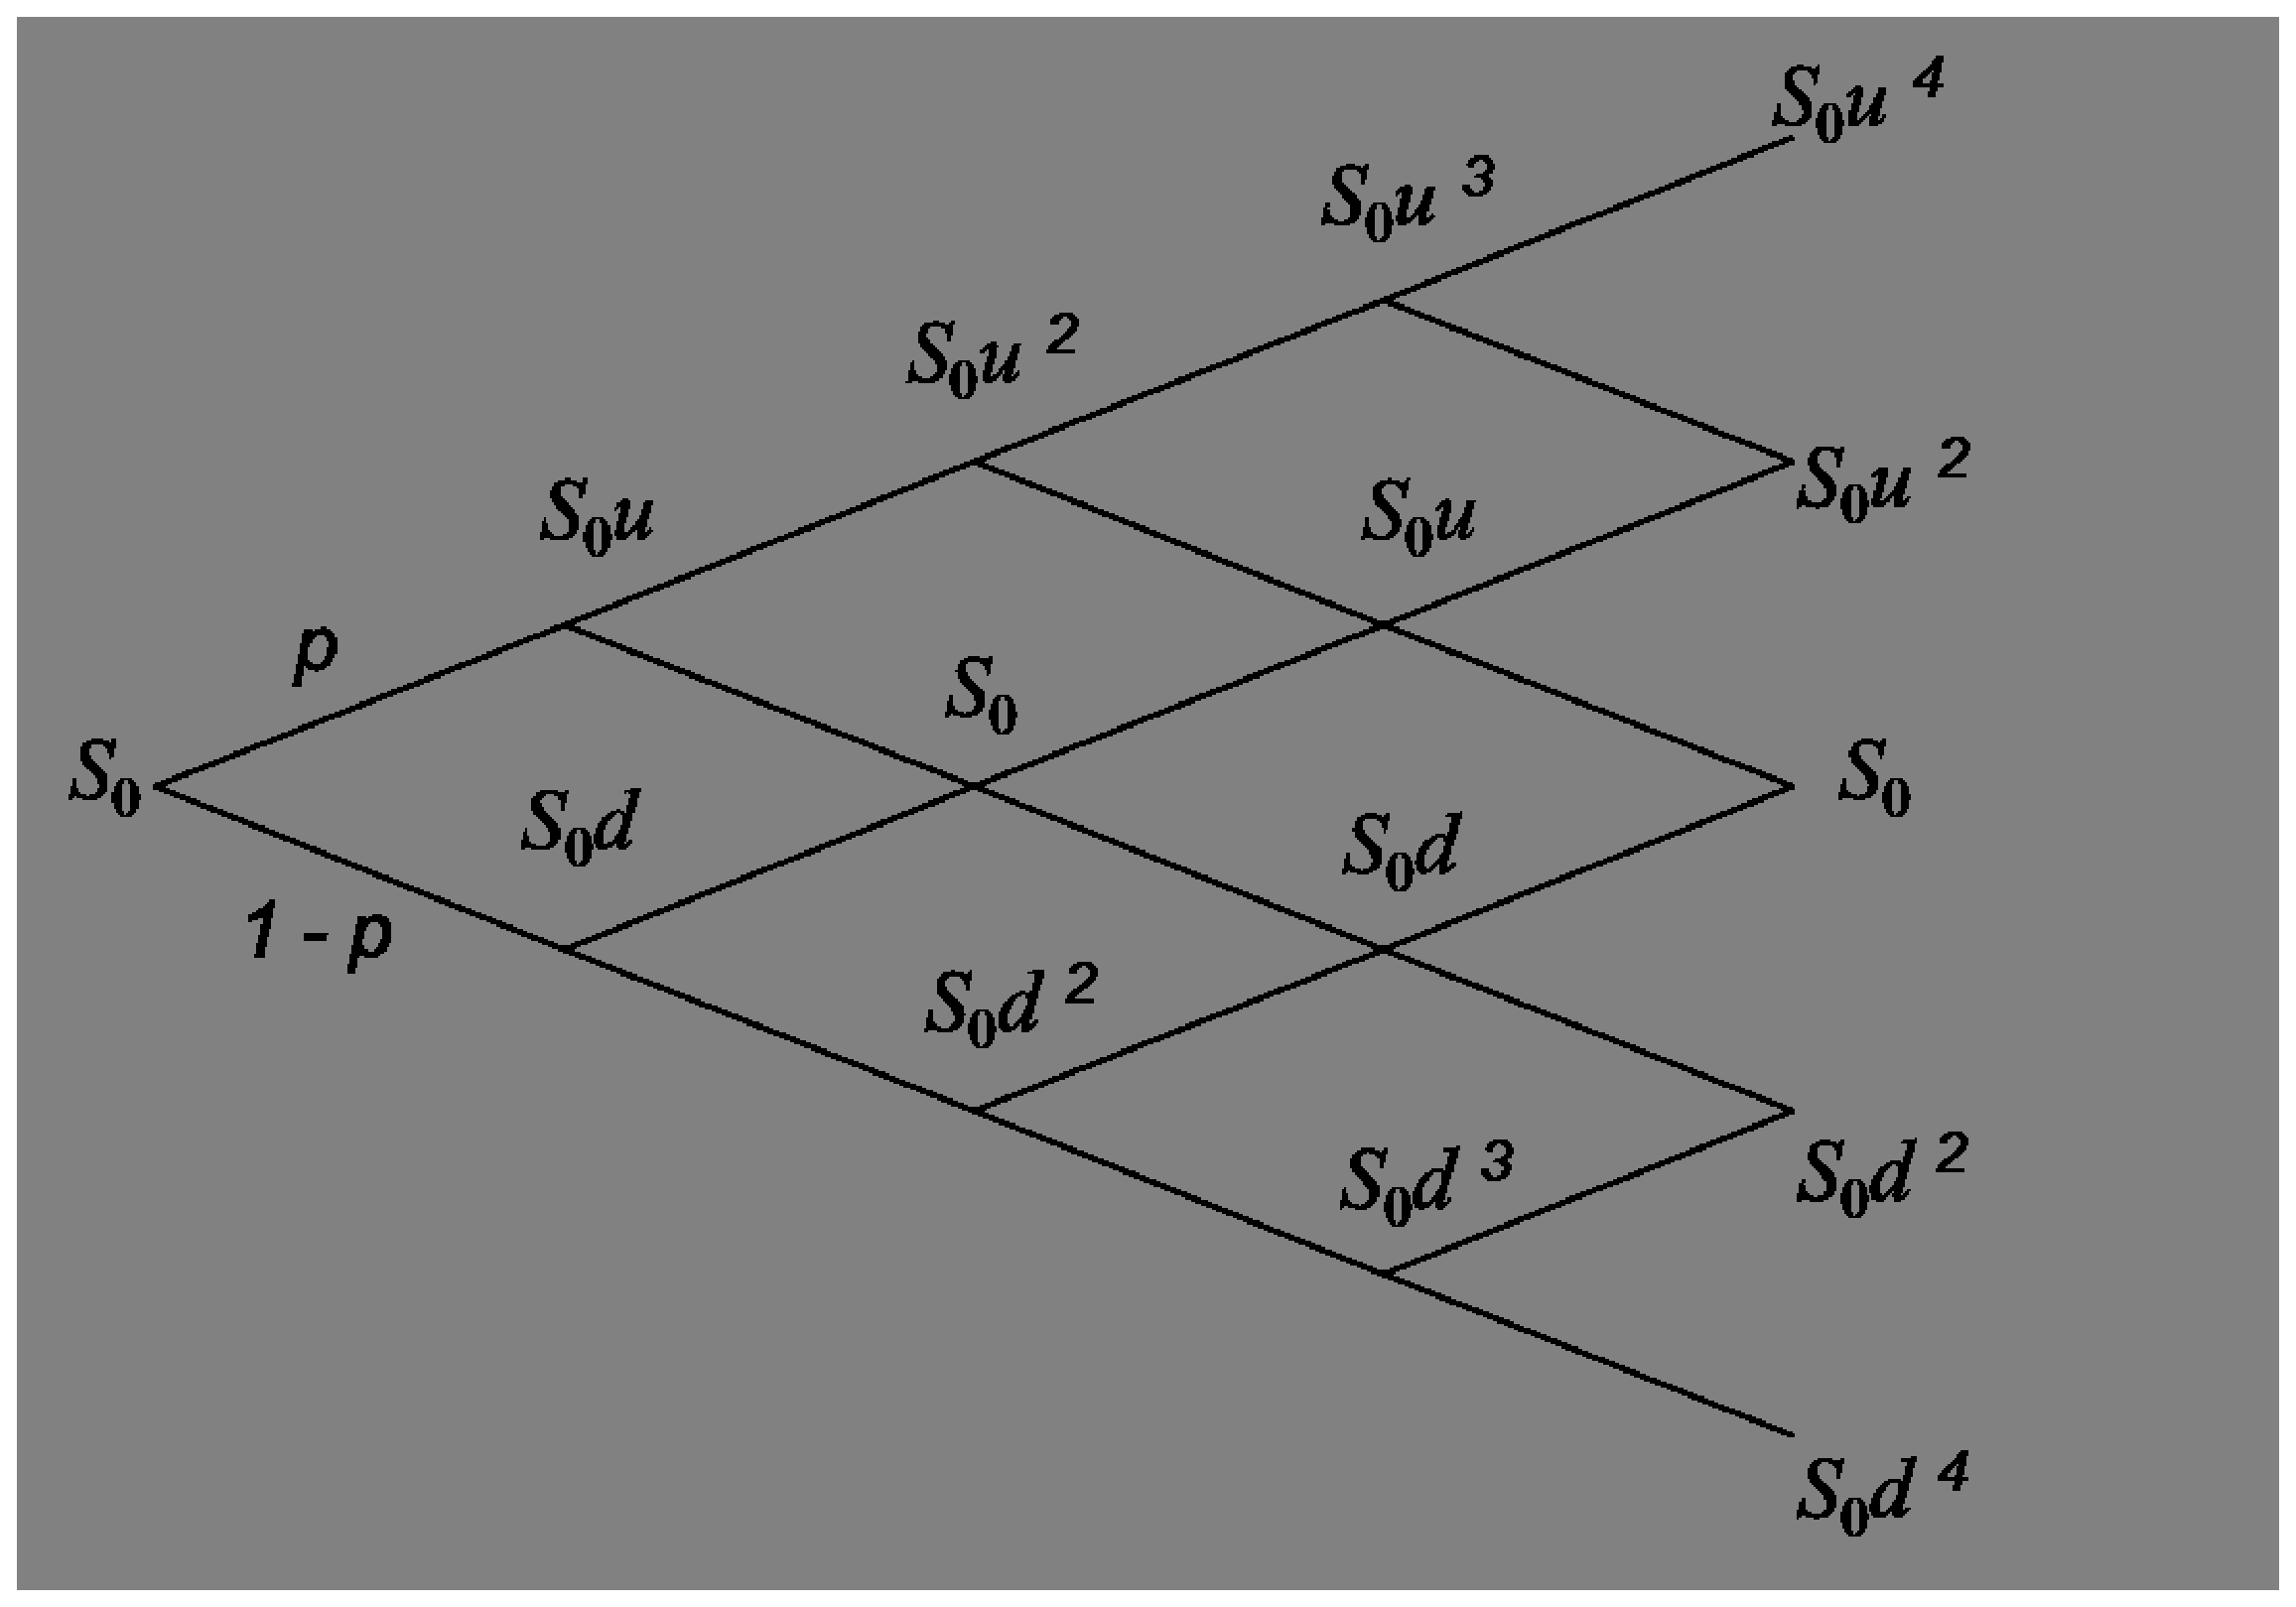
\includegraphics[width=\linewidth]{binomial-tree.eps}
    \caption{The binomial price tree $\mathcal{T}$.}
    \label{fig:binomial_tree}
\end{figure}

\paragraph{Creating the binomial price tree}
The binomial price tree $\mathcal{T}$ of the height $n$ represents the possible future prices within the time period $T$ discretely, as shown in Fig.~\ref{fig:binomial_tree}.
$n$ can be picked arbitrarily. With larger $n$, the result will be more accurate, but the computing overhead will be heavier.
Each node $\mathcal{T}_{t, i}$ is attached with the asset price $S_{t, i}$ and the option price $C_{t, i}$,
where $t \in \{0, \frac{T}{n}, \frac{2T}{n}, \dots, T\}$ is the point of time and $i$ is the number of the node at its level.
The CRR model assumes that the asset price will either move up or down by a specific factor per step in $\mathcal{T}$.
The move-up factor is $u$, and the move-down factor is $d$.
Accordingly, the price after one move-up is $S_{up} = u \cdot S$, and the price after one move-down is $S_{down} = d \cdot S$.

$u$ and $d$ are calculated using the underlying annualized volatility $\sigma_a$ of the asset price:

\begin{align} 
u &= e^{\sigma_a \sqrt{\frac{T}{n}}}\\
d &= e^{- \sigma_a \sqrt{\frac{T}{n}}} = \frac{1}{u}
\end{align}

Here, $T$ is measured in years, and $\sigma_a$ is defined as the standard deviation of the annual price.
$\sigma_a$ can be computed from the daily price standard deviation $\sigma_d$ as below:

\begin{align} 
\sigma_a &= \sigma_d \sqrt{d}\\
\sigma_d &= \sqrt{\frac{\sum^{d}_{i=1} (S_i - \bar{S})^2}{d-1}}
\end{align}

where $d$ is the number of trading days within a year.
For cryptocurrencies, $d$ equals to the number of a days within a year.
Note that $S_i$ is the percentage change of the price on day $i$, rather than the price itself.
$\bar{S}$ is the average value of all $S_i$s within the $d$ days. 

The asset price $S_{t, i}$ can also be computed as $S_{t, i} = S_{0, 1} \cdot u^{N_u - N_d}$, where $S_{0, 1}$ is the spot price, and $N_u, N_d$ are the numbers of move-up and move-down, respectively.

\paragraph{Finding the option price for each leaf node}
In the first step, only the asset prices are determined rather than the option prices.
This step further determines the option prices for leaf nodes.
For each leaf node $\mathcal{T}_{n, i}$, the option price (for Call Options) is $C_{n, i} = max[(S_{n, i} - K), 0]$.

\paragraph{Finding the option prices for earlier nodes}
We back-propagate the option prices for leaf nodes to earlier option prices.
More specifically, the earlier option price is calculated from the option prices of the later two nodes weighted by their state transition possibilities.
The move-up and move-down possibility are $p$ and $q$ where $p + q = 1$, and the risk-free rate is $r = q$.

The earlier option price is calculated from later option prices as:

\begin{align} 
C_{t - \Delta t, i} = e^{-r \Delta t} (p C_{t, i} + q C_{t, i+1})
\end{align}

where $p, q, r$ are computed as


\begin{align} 
p &= \frac{e^{(r-q)\Delta t} - d}{u - d}\\
q &= 1 - p\\
r &= q
\end{align}

such that the related binomial distribution simulates the geometric Brownian motion of the underlying asset value with parameters $r$ and $\sigma$.

For American Options, since the option can be exercised prior to expiry, the option price at each node is

\begin{align}
C_{t - \Delta t, i} = max[e^{-r \Delta t} (p C_{t, i} + q C_{t, i+1}), K]
\end{align}

The earliest option price $S_{0, 1}$ - the estimated option price - can be calculated by iteratively back-propagating the later option prices. 

\subsubsection{Experiments}


\begin{figure}
    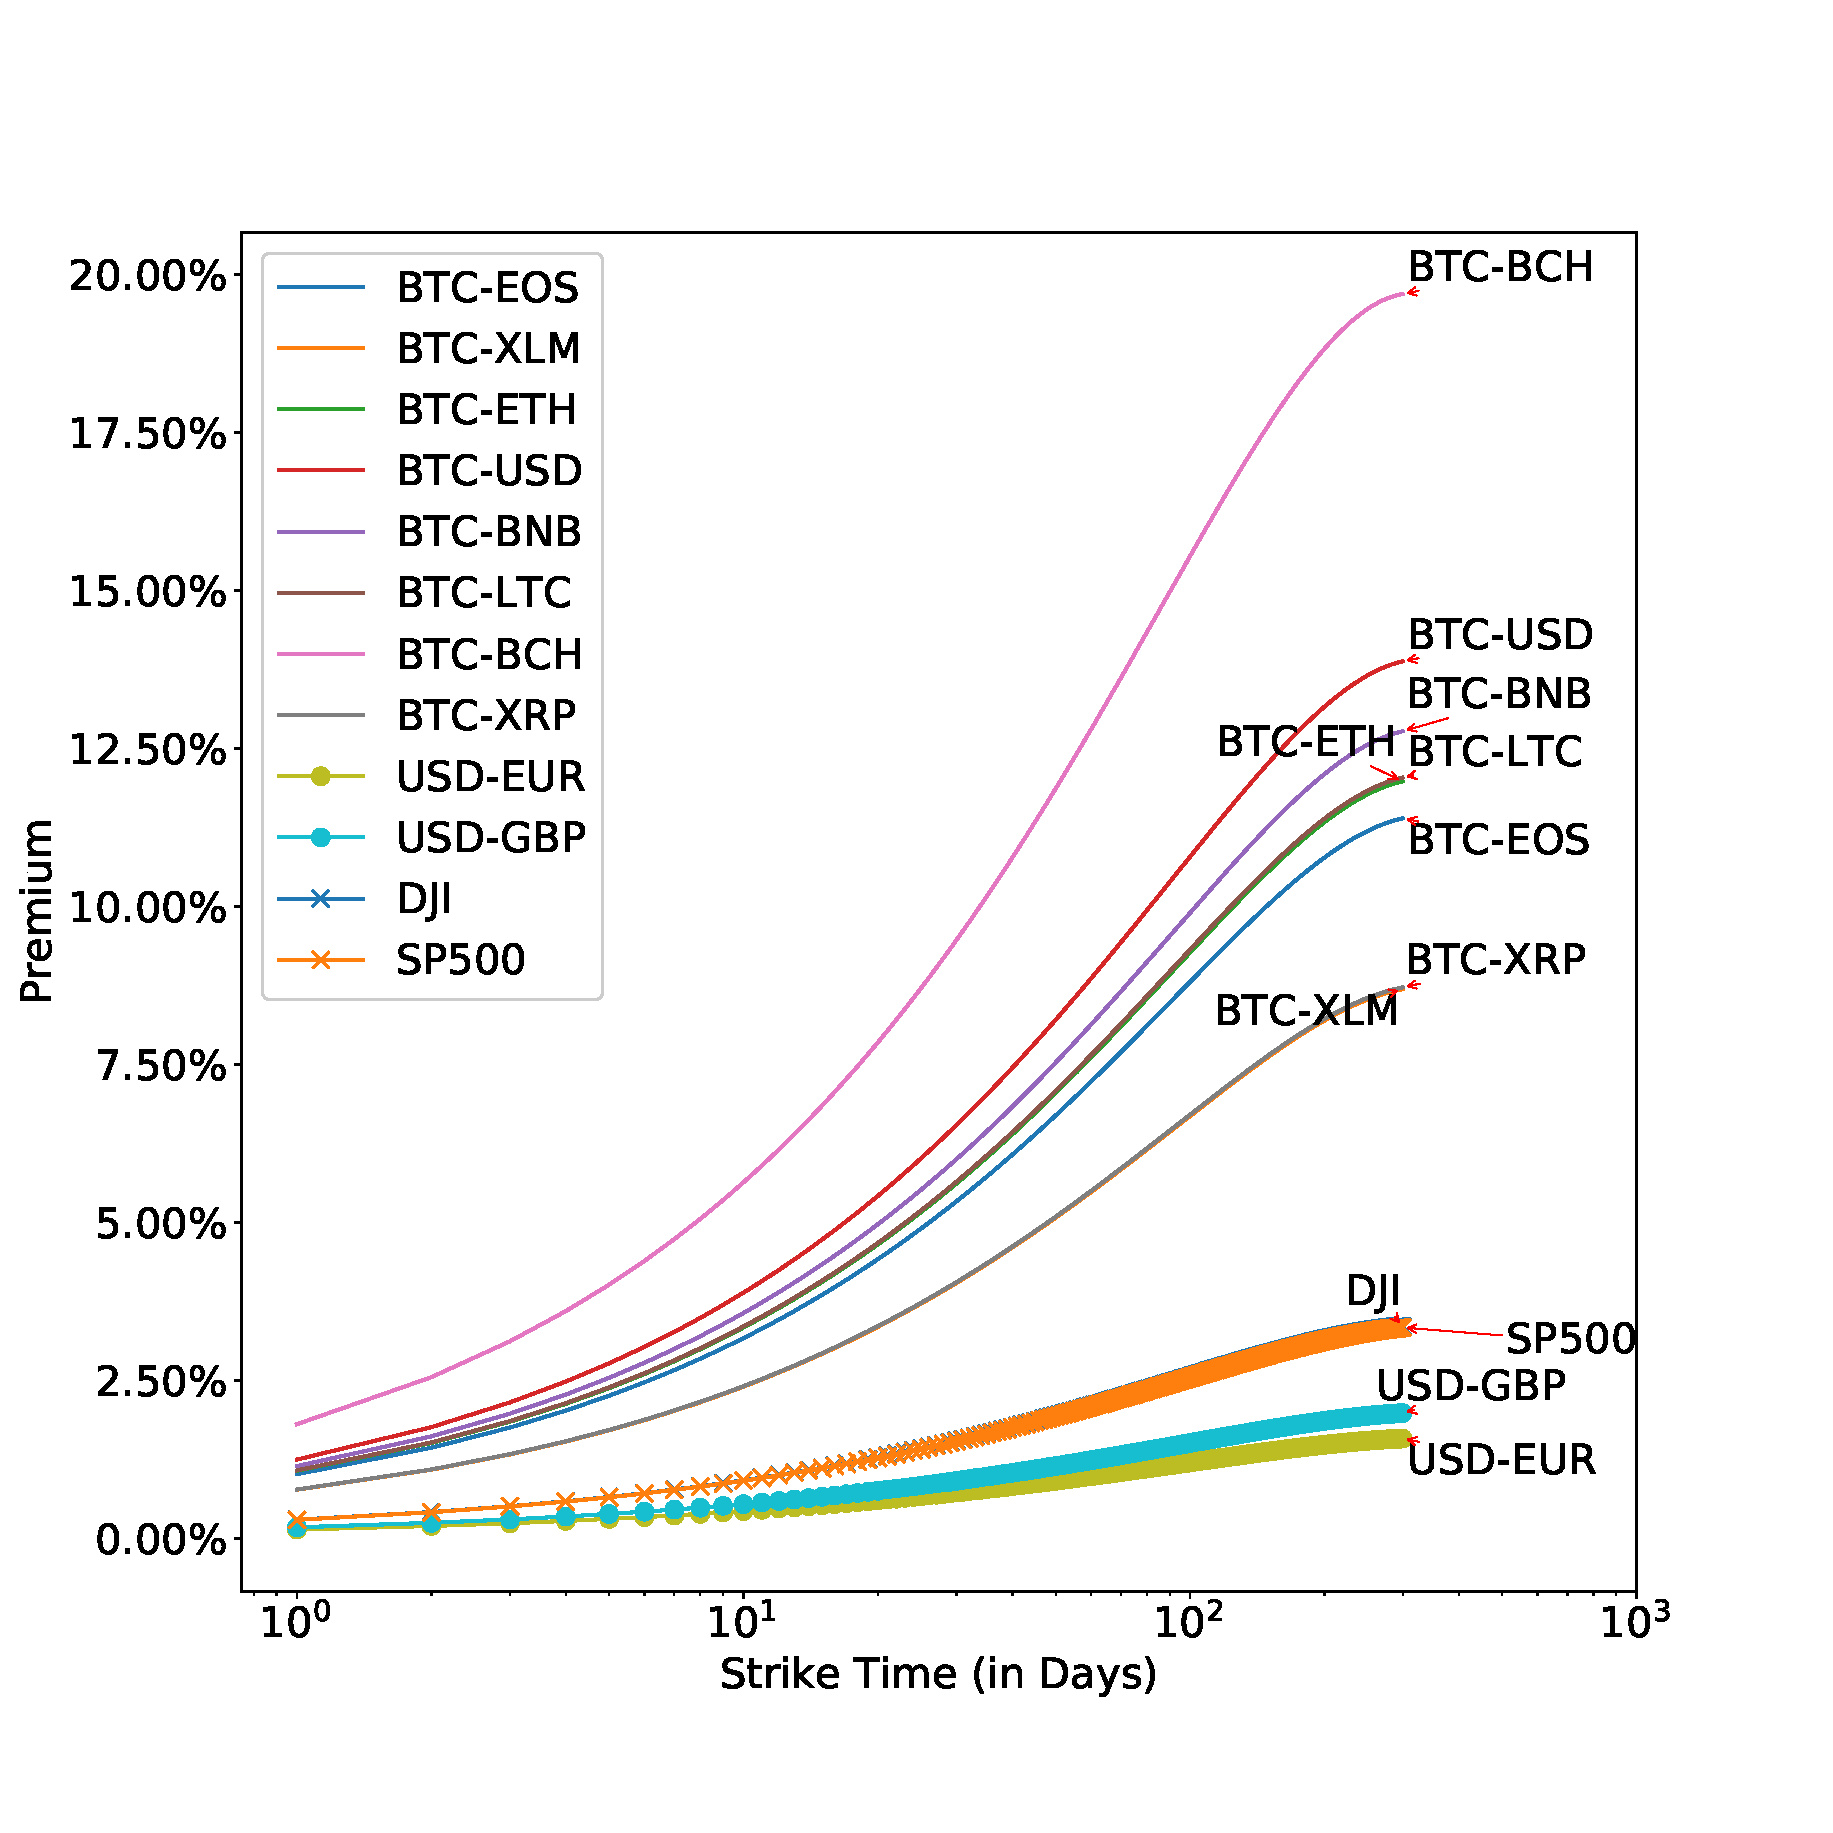
\includegraphics[width=\linewidth]{premium_pricing_result.eps}
    \caption{Estimated premium with different strike times for each cryptocurrency pair, stock index and fiat currency pair. Lines with the marker ``x'' are for stocks; lines with the marker ``o'' are for fiat currencies; and lines without marker are for cryptocurrency pairs.}
    \label{fig:premium_pricing_result}
\end{figure}

We price the same data as Section~\ref{subsec:volatility_analysis} by using the CRR model with $n = 36$ with the strike time $T$ ranging from $1$ to $300$.
Figure~\ref{fig:premium_pricing_result} shows our pricing results.

First, we observe that the premium of cryptocurrency pairs is much more expensive than stocks, and the premium of stocks is more expensive than fiat currencies at any given time.
Recall the evaluated unfairness in Section~\ref{subsec:volatility_analysis}, its results are consistent with the premium pricing results: The higher the volatility is, the more unfair the Atomic Swap will be, and the higher the premium should be.

Second, with the default strike time $T = 1$ of the Atomic Swap, the premium of cryptocurrency pairs vary from approximately 1\% to 2.3\% of the underlying asset value.

Third, for all evaluated items, the premium values rise monotonically.
This is because the longer expiration time lets the option buyer to have more control on the option - He has more time to predict the price and judges whether to exercise the option.